\documentclass{standalone}
\usepackage{tikz}
\begin{document}
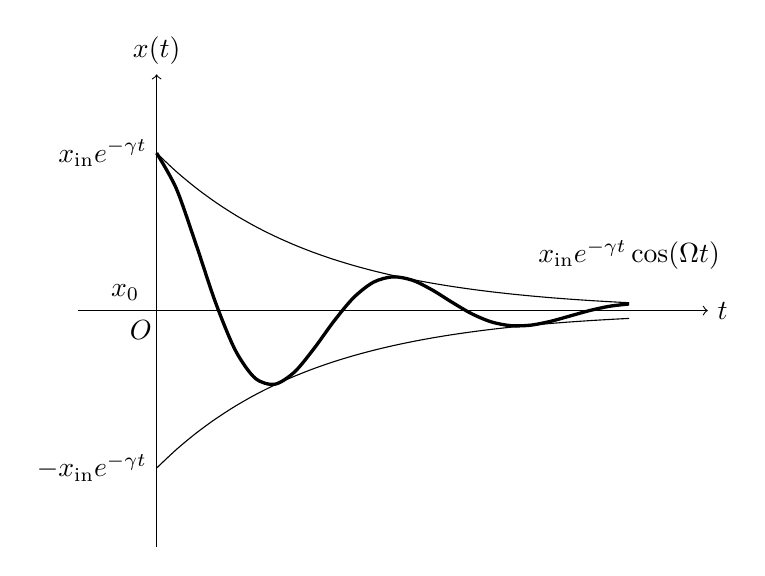
\begin{tikzpicture}[scale=2]
    \draw[->](-0.5,0)--(3.5,0)node[right]{$t$};
    \draw[->](0,-1.5)--(0,1.5)node[above]{$x(t)$};

    \node[above]at(-0.2,0){$x_0$};
    \node[below]at(-0.1,0){$O$};
    
    \node[left]at(0,1){$x_\mathrm{in}e^{-\gamma t}$};
    \node[left]at(0,-1){$-x_\mathrm{in}e^{-\gamma t}$};
    \node[above]at(3,0.2){$x_\mathrm{in}e^{-\gamma t}\cos(\Omega t)$};

    \draw[-]plot[smooth,domain=0:3](\x,{e^-(\x)});
    \draw[-]plot[smooth,domain=0:3](\x,{-e^-(\x)});
    \draw[very thick]plot[smooth,domain=0:3](\x,{(e^-(\x))*cos(4*\x r)});
\end{tikzpicture}
\end{document}